\documentclass[tikz,border=4pt]{standalone}
% Shared style for every figure and for the deck: one accent, one
% highlight, thin lines, rounded nodes, nothing decorative.
\usepackage[T1]{fontenc}
\usepackage{lmodern}
\renewcommand{\familydefault}{\sfdefault}
\usepackage{tikz}
\usetikzlibrary{arrows.meta,positioning,calc,shapes.misc,fit,backgrounds,decorations.pathreplacing}
\definecolor{ink}{RGB}{40,40,40}
\definecolor{soft}{RGB}{150,150,150}
\definecolor{faint}{RGB}{225,225,225}
\definecolor{accent}{RGB}{0,95,115}
\definecolor{accentlight}{RGB}{214,232,236}
\definecolor{warn}{RGB}{196,84,40}
\definecolor{warnlight}{RGB}{247,226,216}
\tikzset{
  every picture/.style={color=ink, line width=0.5pt, font=\small},
  node distance=12mm and 18mm,
  box/.style={draw=ink, rounded corners=2pt, fill=white, inner sep=5pt, minimum height=7mm, align=center},
  maker/.style={box, minimum width=18mm},
  cat/.style={box, inner sep=3.5pt, minimum height=6mm},
  root/.style={box, fill=accentlight, draw=accent},
  bad/.style={box, fill=warnlight, draw=warn},
  ghost/.style={box, draw=soft, text=soft, dashed},
  flow/.style={-{Stealth[length=4pt,width=3.5pt]}, line width=0.5pt},
  sub/.style={-{Stealth[length=4pt,width=3.5pt]}, line width=0.5pt, color=soft},
  strong/.style={flow, color=accent, line width=0.8pt},
  wrong/.style={flow, color=warn},
  lbl/.style={font=\footnotesize, text=ink, inner sep=1.5pt, fill=white},
  note/.style={font=\footnotesize, text=soft, align=center},
  rate/.style={font=\footnotesize, text=accent, inner sep=1pt, fill=white},
}

\usepackage{amsmath}
\usepackage{pgfplots}
\pgfplotsset{compat=1.17}

\begin{document}
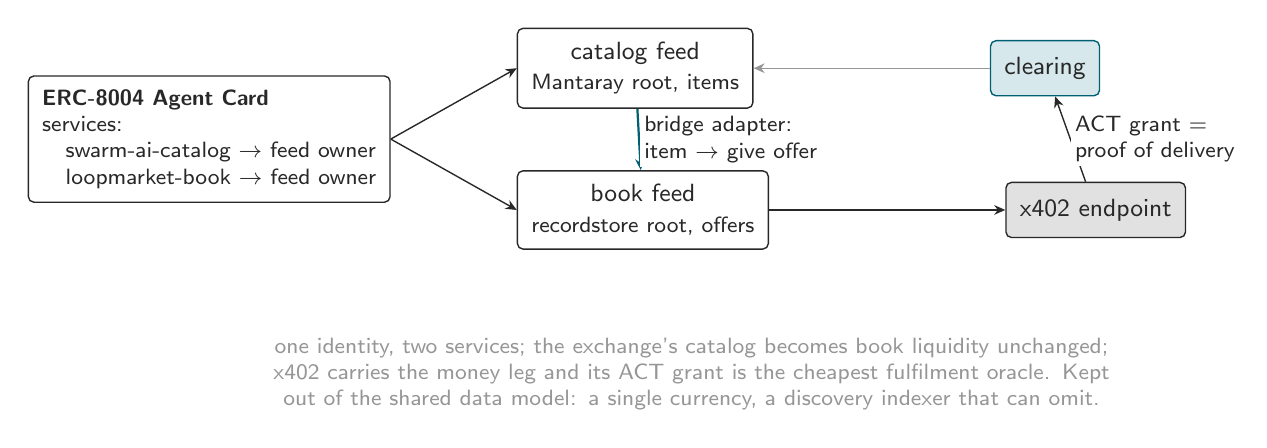
\begin{tikzpicture}[node distance=6mm and 16mm]
  \node[box, align=left, font=\footnotesize] (card) {\textbf{ERC-8004 Agent Card}\\ services:\\ \quad swarm-ai-catalog $\to$ feed owner\\ \quad loopmarket-book $\to$ feed owner};
  \node[box, right=of card, yshift=9mm] (cat) {catalog feed\\{\footnotesize Mantaray root, items}};
  \node[box, right=of card, yshift=-9mm] (book) {book feed\\{\footnotesize recordstore root, offers}};
  \draw[flow] (card.east) -- (cat.west); \draw[flow] (card.east) -- (book.west);
  \draw[strong] (cat) -- node[lbl, right, align=left] {bridge adapter:\\ item $\to$ give offer} (book);
  \node[box, right=30mm of book, fill=faint] (x) {x402 endpoint};
  \node[root, right=30mm of cat] (set) {clearing};
  \draw[flow] (book) -- (x);
  \draw[flow] (x) -- node[lbl, right, align=left] {ACT grant =\\ proof of delivery} (set);
  \draw[sub] (set) -- (cat);
  \node[note, text width=120mm, anchor=north west] at (0,-24mm) {one identity, two services; the exchange's catalog becomes book liquidity unchanged; x402 carries the money leg and its ACT grant is the cheapest fulfilment oracle. Kept out of the shared data model: a single currency, a discovery indexer that can omit.};
\end{tikzpicture}
\end{document}
